\subsection{Research setting}
    % what are the contests like, what kind of configuration settings are available? % TODO consider if needed
    % Contests hosted in Choicely can be divided into generally two groups:
    
    % \begin{enumerate}
    %     \item voting contests: the contest organizer provides the participants to the contest. This way the list of participants cannot be changed as soon as a contest is created.
    %     \item challenge contests: the public provides the participants to the contest. The list of participants may change over time depending on how many users would like to join with their own content. 
    % \end{enumerate}
    
    % From the viewpoint of this research, the contest types are not influential, because it is not studied how users participate into contests. Instead, the focus is put on studying the voting behavior of the public based on their demographic attributes. This aspect is independent from the type of the contests, however it would be interesting to study the platform from this aspect in another study.

    % The contests in the platform are created by users or brands. % TODO consider if needed

    % voting options
    Various voting options are available for contests. The author of the contest has the choice of setting a limit on how many votes users can spend on individual participants or the whole contest in overall. For instance, if the maximum votes in the contest is set to 1, users can give exactly one vote on one and only one participant. Configuration settings allow infinite votes as well. For instance, users may vote on all of the participants as many times as they like in a talent show in this case. Removing votes is possible, if the author has decided to enable this possibility. Votes cannot be modified after the contest has ended. Each contest has its own voting configuration. 
    
    % free-silver-gold votes
    On top of the regular free votes, contest authors may allow users to earn more votes (called "silver votes") by sharing the contest on social media or by watching advertisements. Furthermore, contest authors can allow users to purchase more votes (called "star votes" or "gold votes") with exactly the same restriction settings as explained above. Note, however that the configuration for the three vote types are distinct for every contest. This means that the limitation on free/silver/star votes may differ for individual participants as well as the whole contest. For instance, a contest author may allow users to spend only 5 votes for free, but unlimited number of silver and gold votes in a contest.

    % Each user profile contains the features listed in Table \ref{user_profile_fields}. % TODO consider removing

    % \begin{table}[]
    %     \centering
    %     \begin{tabular}{l|l}
    %         \textbf{Field}              & \textbf{Type} \\
    %         \hline
    %         Full name                   & Free text \\
    %         Profile picture             & Image \\ 
    %         Cover image                 & Image \\
    %         Gender                      & Male/Female/Other/Not specified \\
    %         Location                    & Country, state and city \\
    %         Birthday                    & Datetime \\ 
    %         Age group                   & 0-17/18-24/25-34/35-44/45-54/55-64/65+ \\
    %         Introduction/Bio            & Free text
    %     \end{tabular}
    %     \caption{The list of fields and their types for each user profile.}
    %     \label{user_profile_fields}
    % \end{table}  

    % what kind of data is generated?
    Consequently, the available data is two-folded: the user profiles contain demographic information about the users (age group, gender and location), while contests have a number of participants with arbitrary number of votes that the users have spent on them. The latter kind of data can be seen as digital footprints generated by users in the Choicely platform. The combination of these datasets sums up to the user data as explained in the previous chapter and Figure \ref{user_data_venn} in this particular case. This is further supported with the meta data of contests explained in the previous paragraph. 

    %The vote changes for the contests are stored as transactions. This means that the database contains not the final results of the voting, but rather the changes what users made while using the software. This way it is possible to analyze the votes over time and to look at changes individually. For instance, it is possible to tell if a user has removed his/her votes from participant A and moved them to participant B. Furthermore, this way of data representation to restore or simulate any previous state of the contest, in case it would be needed.

    % why is the data analysis relevant from scientific research point of view?
    Performing scientific research on such data is interesting for multiple reasons. To begin with, at the time of this research Choicely did not utilize data analysis tools to gain better understanding on the collected data. It is in the interest of the company and its customers to better understand what kind of audience was engaged in the past, what kind of content is more (or less) successful and what tendencies in user behavior can be extracted from the data. As a result, the introduction of data analysis and visualization tools at the company will greatly enhance business value of the firm, provide deeper understanding on the domain as well as the existing user base.   
    
    % how is Choicely different than other social networks or any other repository of user data?
    Secondly, Choicely can be looked at as a social network, because some of the pictures uploaded to the platform is generated by users. Users also have the possibility to express their appreciation or support towards some contest participants by spending votes on them. Similarly to social networking sites, where the "like" feature is often used \cite{jang2015noreciprocity, bakhshi2014faces} this phenomena can be looked at as a way of expressing personal opinion. 
    
    In comparison to most of the currently available social networks, voting platforms like Choicely are observed by the audience differently. On one hand, social media sites usually list posts or images on a feed, where there is theoretically no relation between the posts that follow eachother. % TODO citation
    On the other hand, contestants in the Choicely platform share similarities as they were nominated for the same contest. Accordingly, there must be some similarity among them as all are subjects of the contest's topic, rules and are competing for the best possible result. 

    % so what? Why is that important from user point of view
    This slight difference can make a big change in terms of user behavior. The focus moves from "what kind of content I like" to "which piece of content I like the most in comparison to the rest". Consequently, users will scan through some (or optimally all) of the contestants and make unconscious decisions upon whether to give vote(s) on certain contest participant(s). The users express their favour and support towards a subset of contenders, hence helping them to reach their ultimate goal: winning the contest. 
    % how can this contribute to user behavior and social media studies? 
    This uniqueness compared to other social networking sites offers a great possibility for research. Therefore, the hands-on goals towards the analysis are two-folded: 

    \begin{enumerate}
        \item identifying what kind of images among different contests users like, and
        \item what kind of content similar group of users like.
    \end{enumerate}

    % how computer vision is going to be utilized? 
    One of the challenges in connecting users with topics is that there is no indication on what the content on the participants' pictures is. Contest authors only assign categories to the contests to be created, which does not necessarily describe the entrants. Other researches have successfully utilized computer vision to gather meta data for the uploaded content in image sharing communities \cite{bakhshi2014faces, hu2014we}. 
    
    % what is the solution to this problem?
    Deriving from the success in previous studies \cite{hu2014we, farseev2015harvestingmultiplesources, han2016teensarefrommars, bakhshi2014faces}, computer vision is applied in this research to identify labels that appear on the participants' images. For instance, a beauty pageant's entry image may be labelled with meta data, such as "Beauty", "Photo Shoot", "Smile" and "Blonde". Similarly, a design contest entry might have topic labels, such as "Landmark" or "Architecture". Figure \ref{google_vision_labels} displays an example, where the Google Vision API was used to extract labels from images which were used in contests of Choicely.

    \begin{figure}[h] 
		\begin{center}
            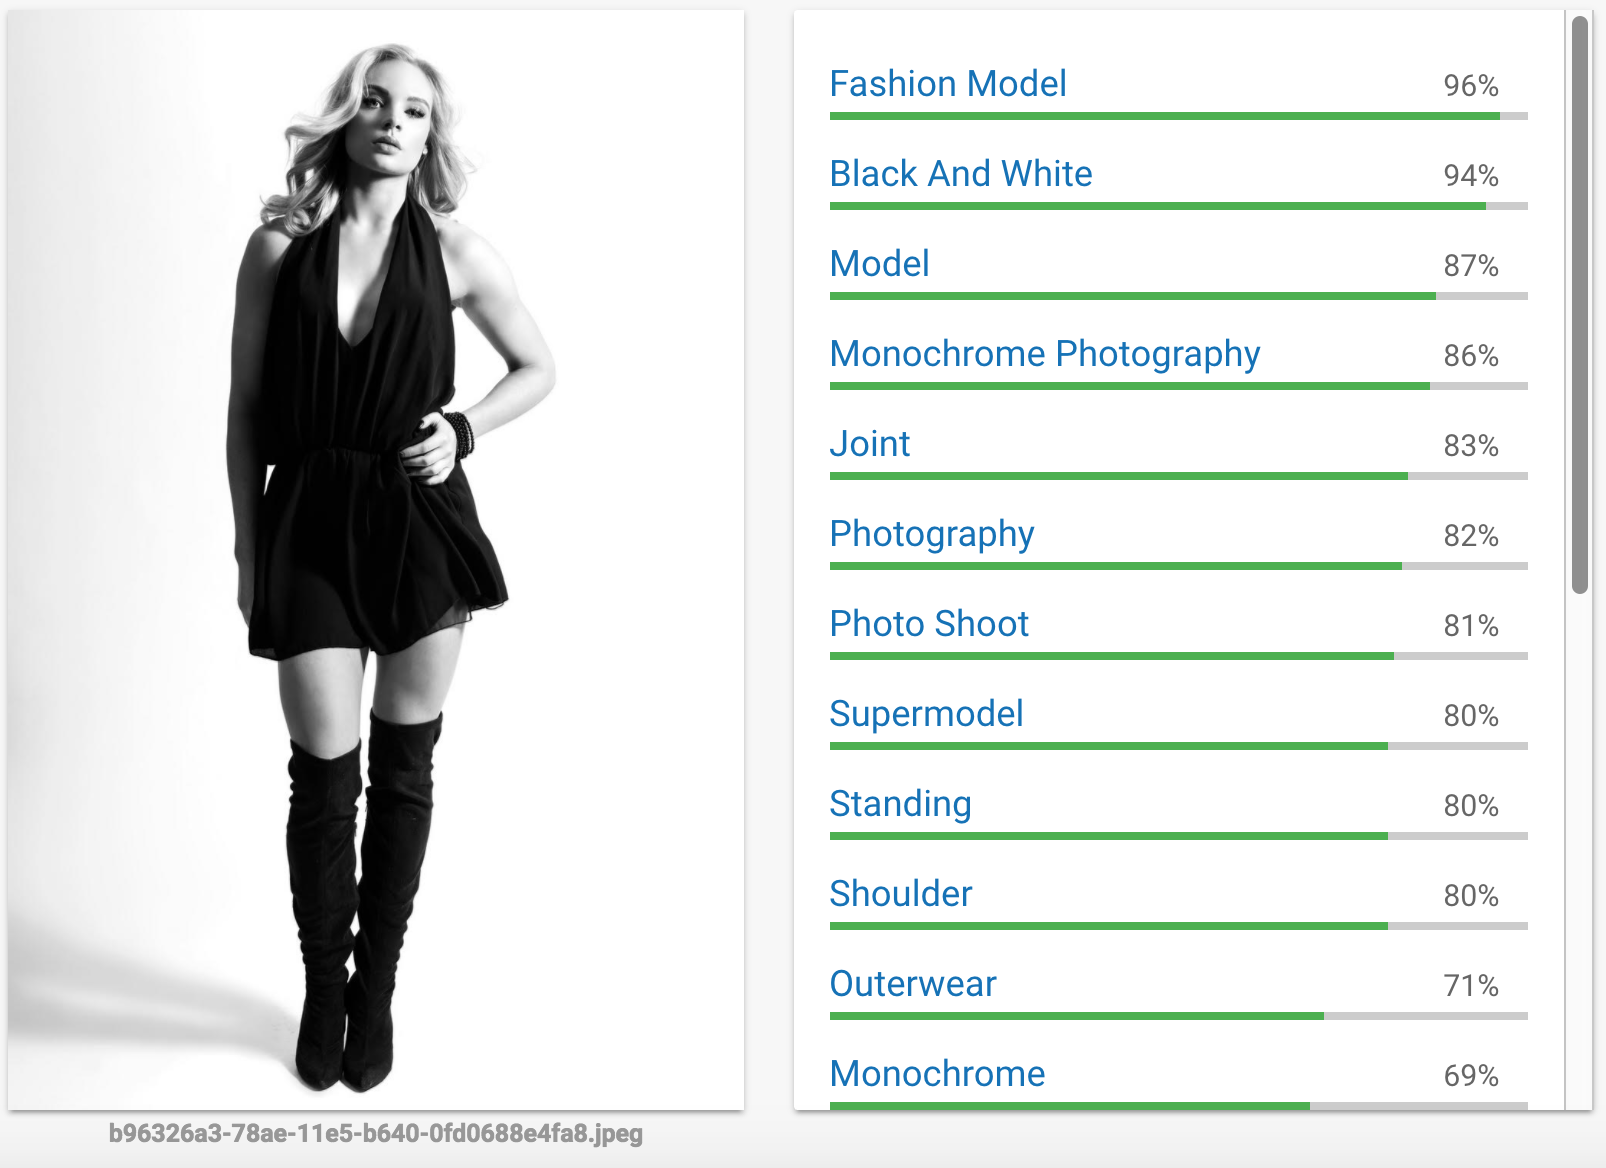
\includegraphics[width=0.8\textwidth]{images/google_vision_labels.png}
            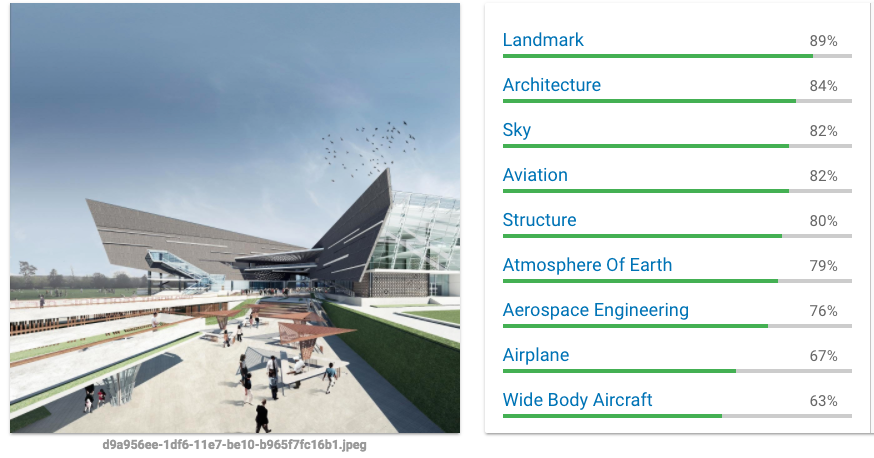
\includegraphics[width=0.8\textwidth]{images/google_vision_labels2.png}
			\caption{The labels identified by the Google Vision API on two of the contest participant's images.}
			\label{google_vision_labels}
		\end{center}
    \end{figure}

    % how are the labels used - what is the method performed on them? 
    Combining the identified labels and the vote data can provide information on user behavior. For instance it can be identified which demographic group of users like what kind of content, or the behavioral differences between two or more groups can be compared to eachother. Furthermore, this kind of information could be used to recommend new content in the platform to users which they have not seen before. Last but not least, it could be identified that which traits of participants contribute to more votes and engagement by users or certain user groups.  
    
    \subsection{Data structure and retrieval}
    % architectural overview
    In order to better understand the data, the data structure and the architecture of the Choicely platform is explained briefly in this chapter. Most of the platform's data is stored currently in the Google Cloud Platform\footnote{\url{https://cloud.google.com}}, more specifically in Google Datastore\footnote{\url{https://cloud.google.com/datastore}} and Google BigQuery\footnote{\url{https://cloud.google.com/bigquery}}. Google Vision\footnote{\url{https://cloud.google.com/vision/}} is utilized as a computer vision service to gather the meta data for the contestants' images. 
    
    Google Datastore is highly scalable document database which is built on top of NoSQL technology \cite{google-datastore-overview}. By providing flexible storage, performant computing resources, encryption possibilities and high availability, the service can serve wide range of applications and various type of business data of companies \cite{google-datastore-overview}. Google BigQuery is a data warehouse for enterprise purposes, large-scale data storage, processing and analysis \cite{google-bigquery-overview}. Most of Choicely's data is stored in Google Datastore, however the computer-vision identified tags of the participants' images (Figure \ref{google_vision_labels}) are located in Google BigQuery at the present time.
    
    The data is structured into entities in both Datastore and BigQuery. There is parent-child connection between entities, which are key for the retrieval of some of the unique entities. For instance, contests belong to Users or Brands (as content providers), which are separate entities in the platform. Certain entities can be identified by multiple parent entities. Entities that have no parent(s) can be identified with their unique identifiers and indexed with some other fields. For example, users can be filtered by gender and age group, or unique identifier. 
    
    The data is generated by content providers, who create contests in the platform and users, who cast votes on their favorite participant(s) in the contests through one of the interfaces explained in Figure \ref{choicely_platforms}. The contest participants' images are identified automatically via the combination of Google Vision \footnote{\url{https://cloud.google.com/vision/}} and Google Cloud Functions \footnote{\url{https://cloud.google.com/functions/}} once they are uploaded to the database. Google Vision is another component of the Google Cloud, which provides powerful image analysis solutions for software developers \cite{google-vision-overview}. In this study, the usage of this component is limited to the classification of the content on the images as explained above.  Google Cloud Functions \footnote{\url{https://cloud.google.com/functions/}} are used to be able to automatically assign the labels to the images so that the manual work can be reduced to the least minimum. 

    Similarly to SQL join statements, the aforementioned identifiers and the parent-child relationship can be used to join list of various entities together. This property is used to aggregate and prepare data for the purposes of the analyses to be performed. Accordingly, the Contest, User, ContestVote, Vote and ImageLabel entities are joined together via their connections to construct the data structure displayed in Table \ref{association_analyisis_data}. This data structure establishes the basis of the Association Analysis, which is performed to address RQ3. 

    \begin{figure}[h] 
		\begin{center}
            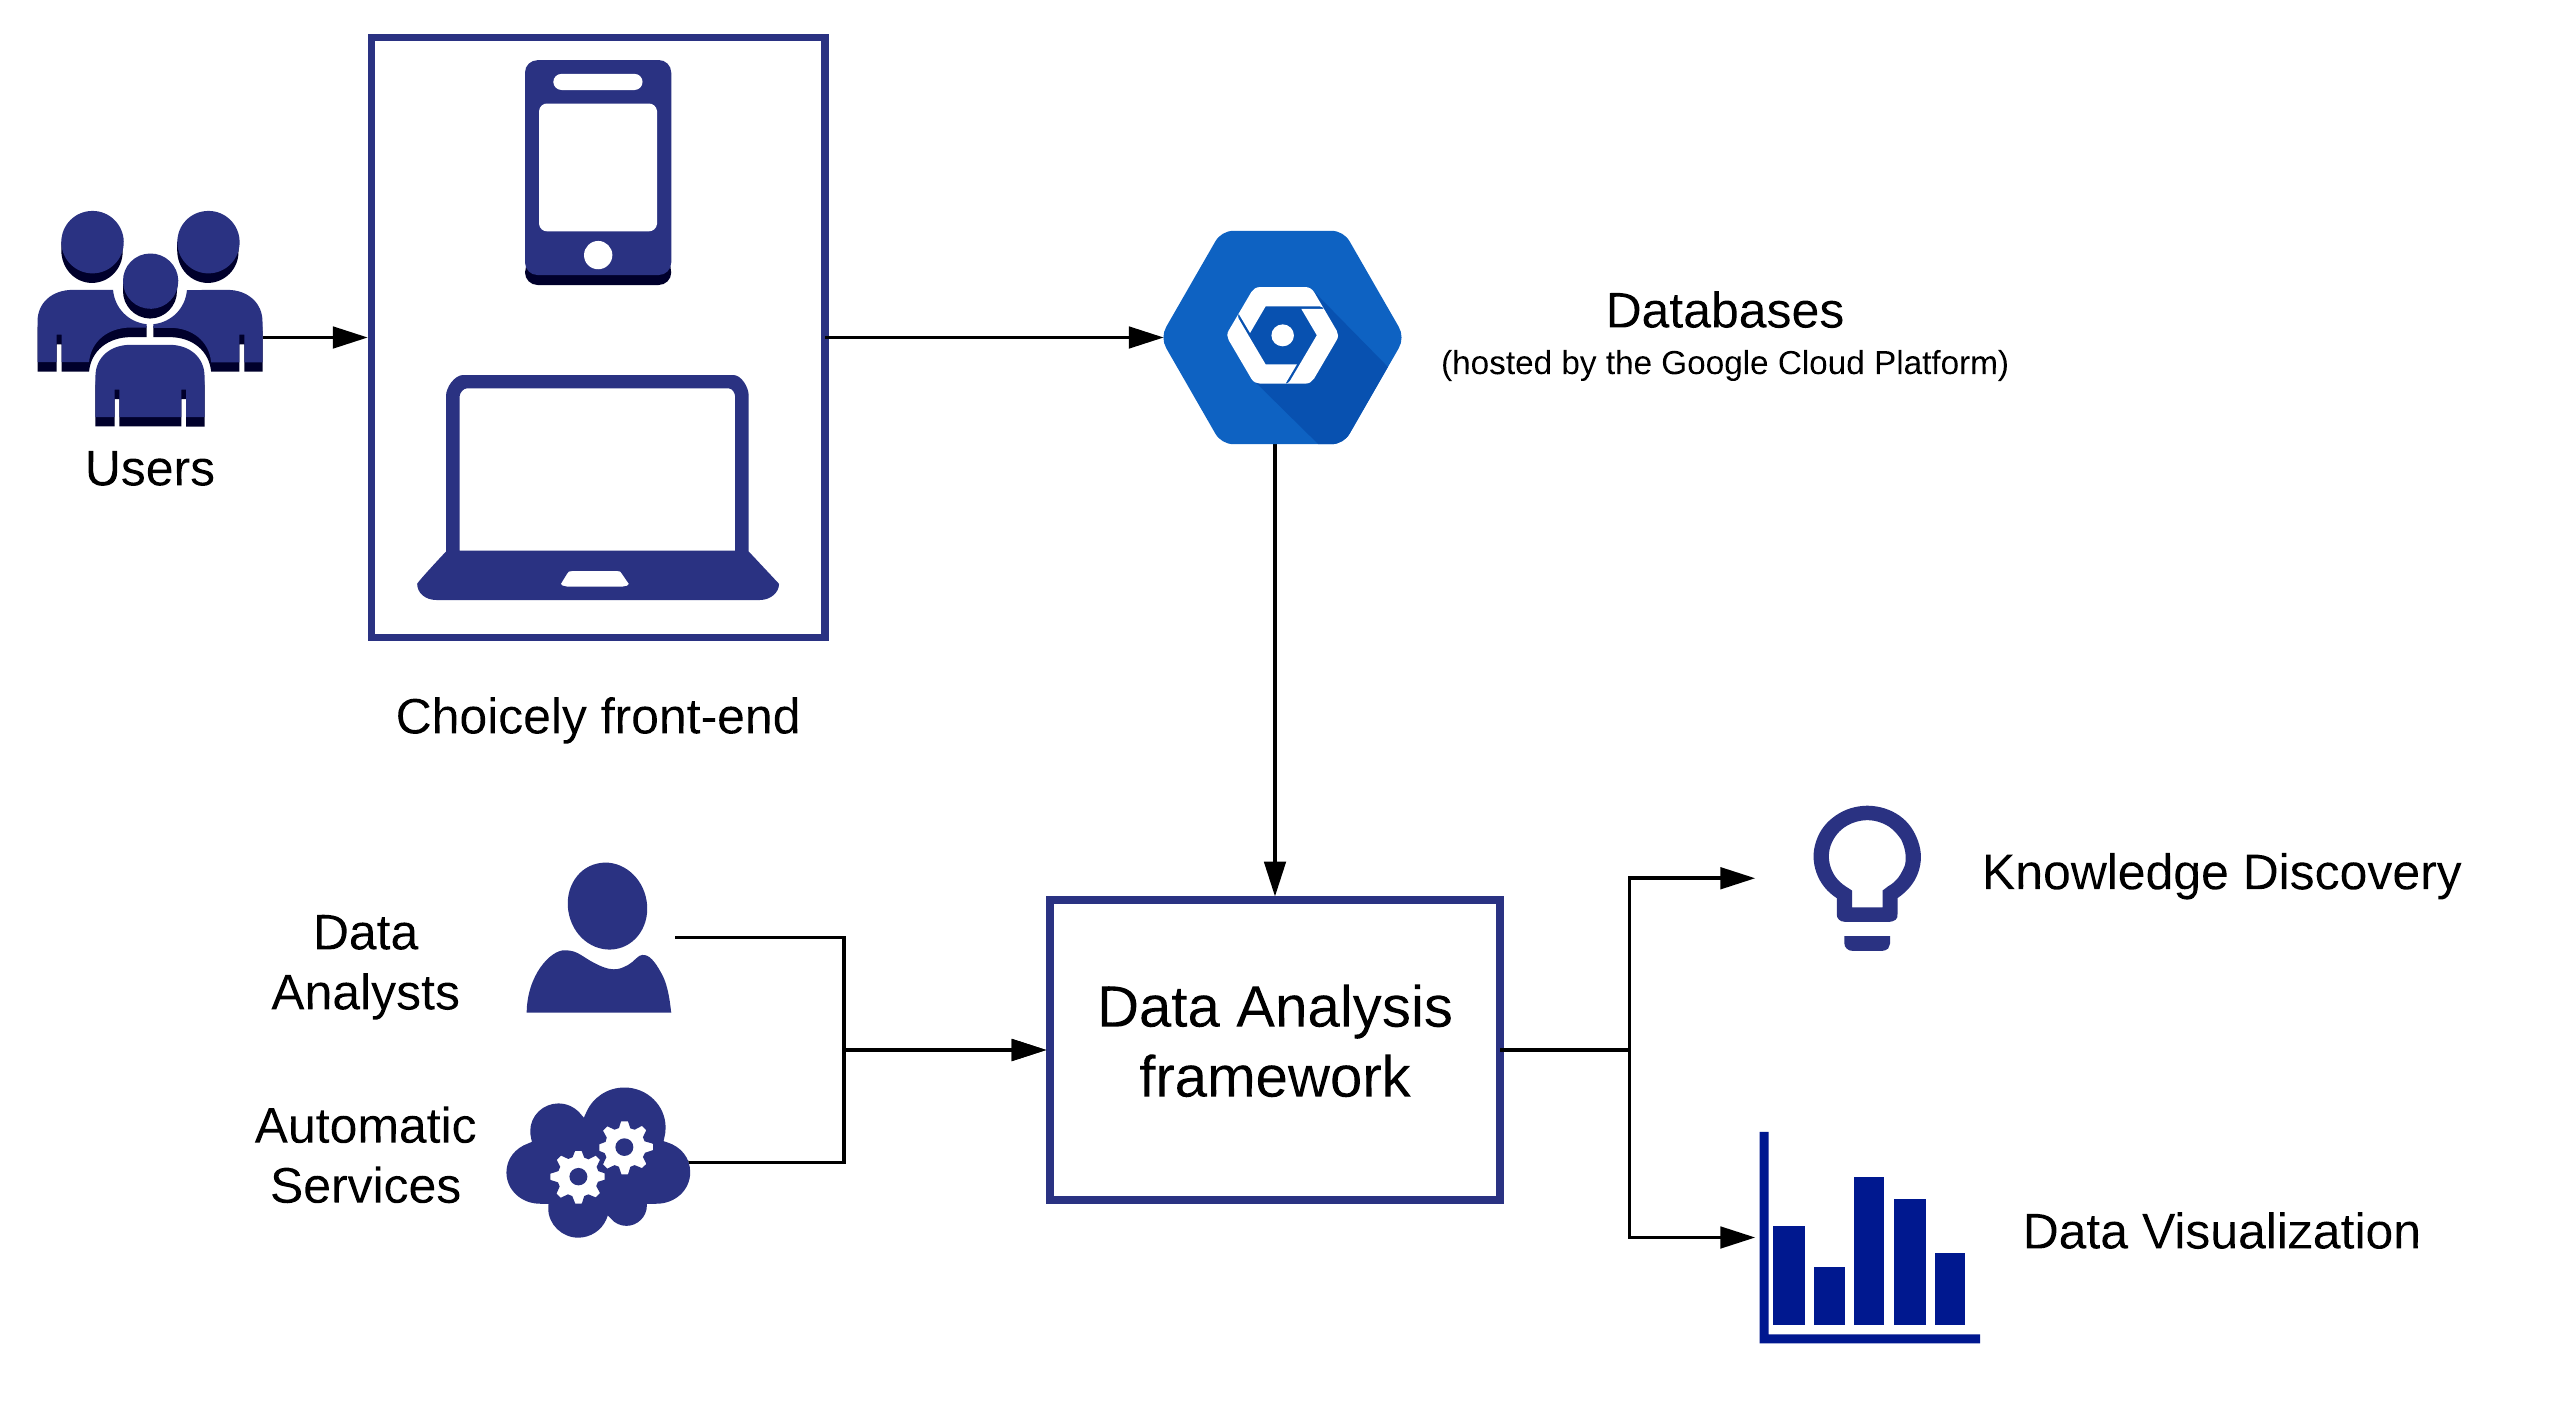
\includegraphics[width=0.8\textwidth]{Images/architecture.png}
			\caption{The brief architectural overview of the Choicely platform.}
			\label{choicely_architecture}
		\end{center}
    \end{figure}

    Figure \ref{choicely_architecture} displays the architecture of the Choicely platform on a high level. The Users of the system use the Choicely clients on their mobile or personal computer to create new contests or cast votes in the existing ones. 
    % From the point of view of this thesis work there are no significant differences between the two entitites, their role is simply to provide engaging content to a large number of users. Users then on the other hand participate in the contests by casting votes on the contest participants. 
    The Vote and Contest data is collected and stored to the databases that are hosted by Google Datastore. The data analysis is then performed by the Data Analysis framework, which is used by either a data analyst or an automatic service. This thesis work is devoted to establish the core functionality of this framework through this thesis work. Finally, Knowledge Discovery and Data Visualization is performed on the output of the framework. 
    
    % \begin{figure}[h] 
	% 	\begin{center}
    %         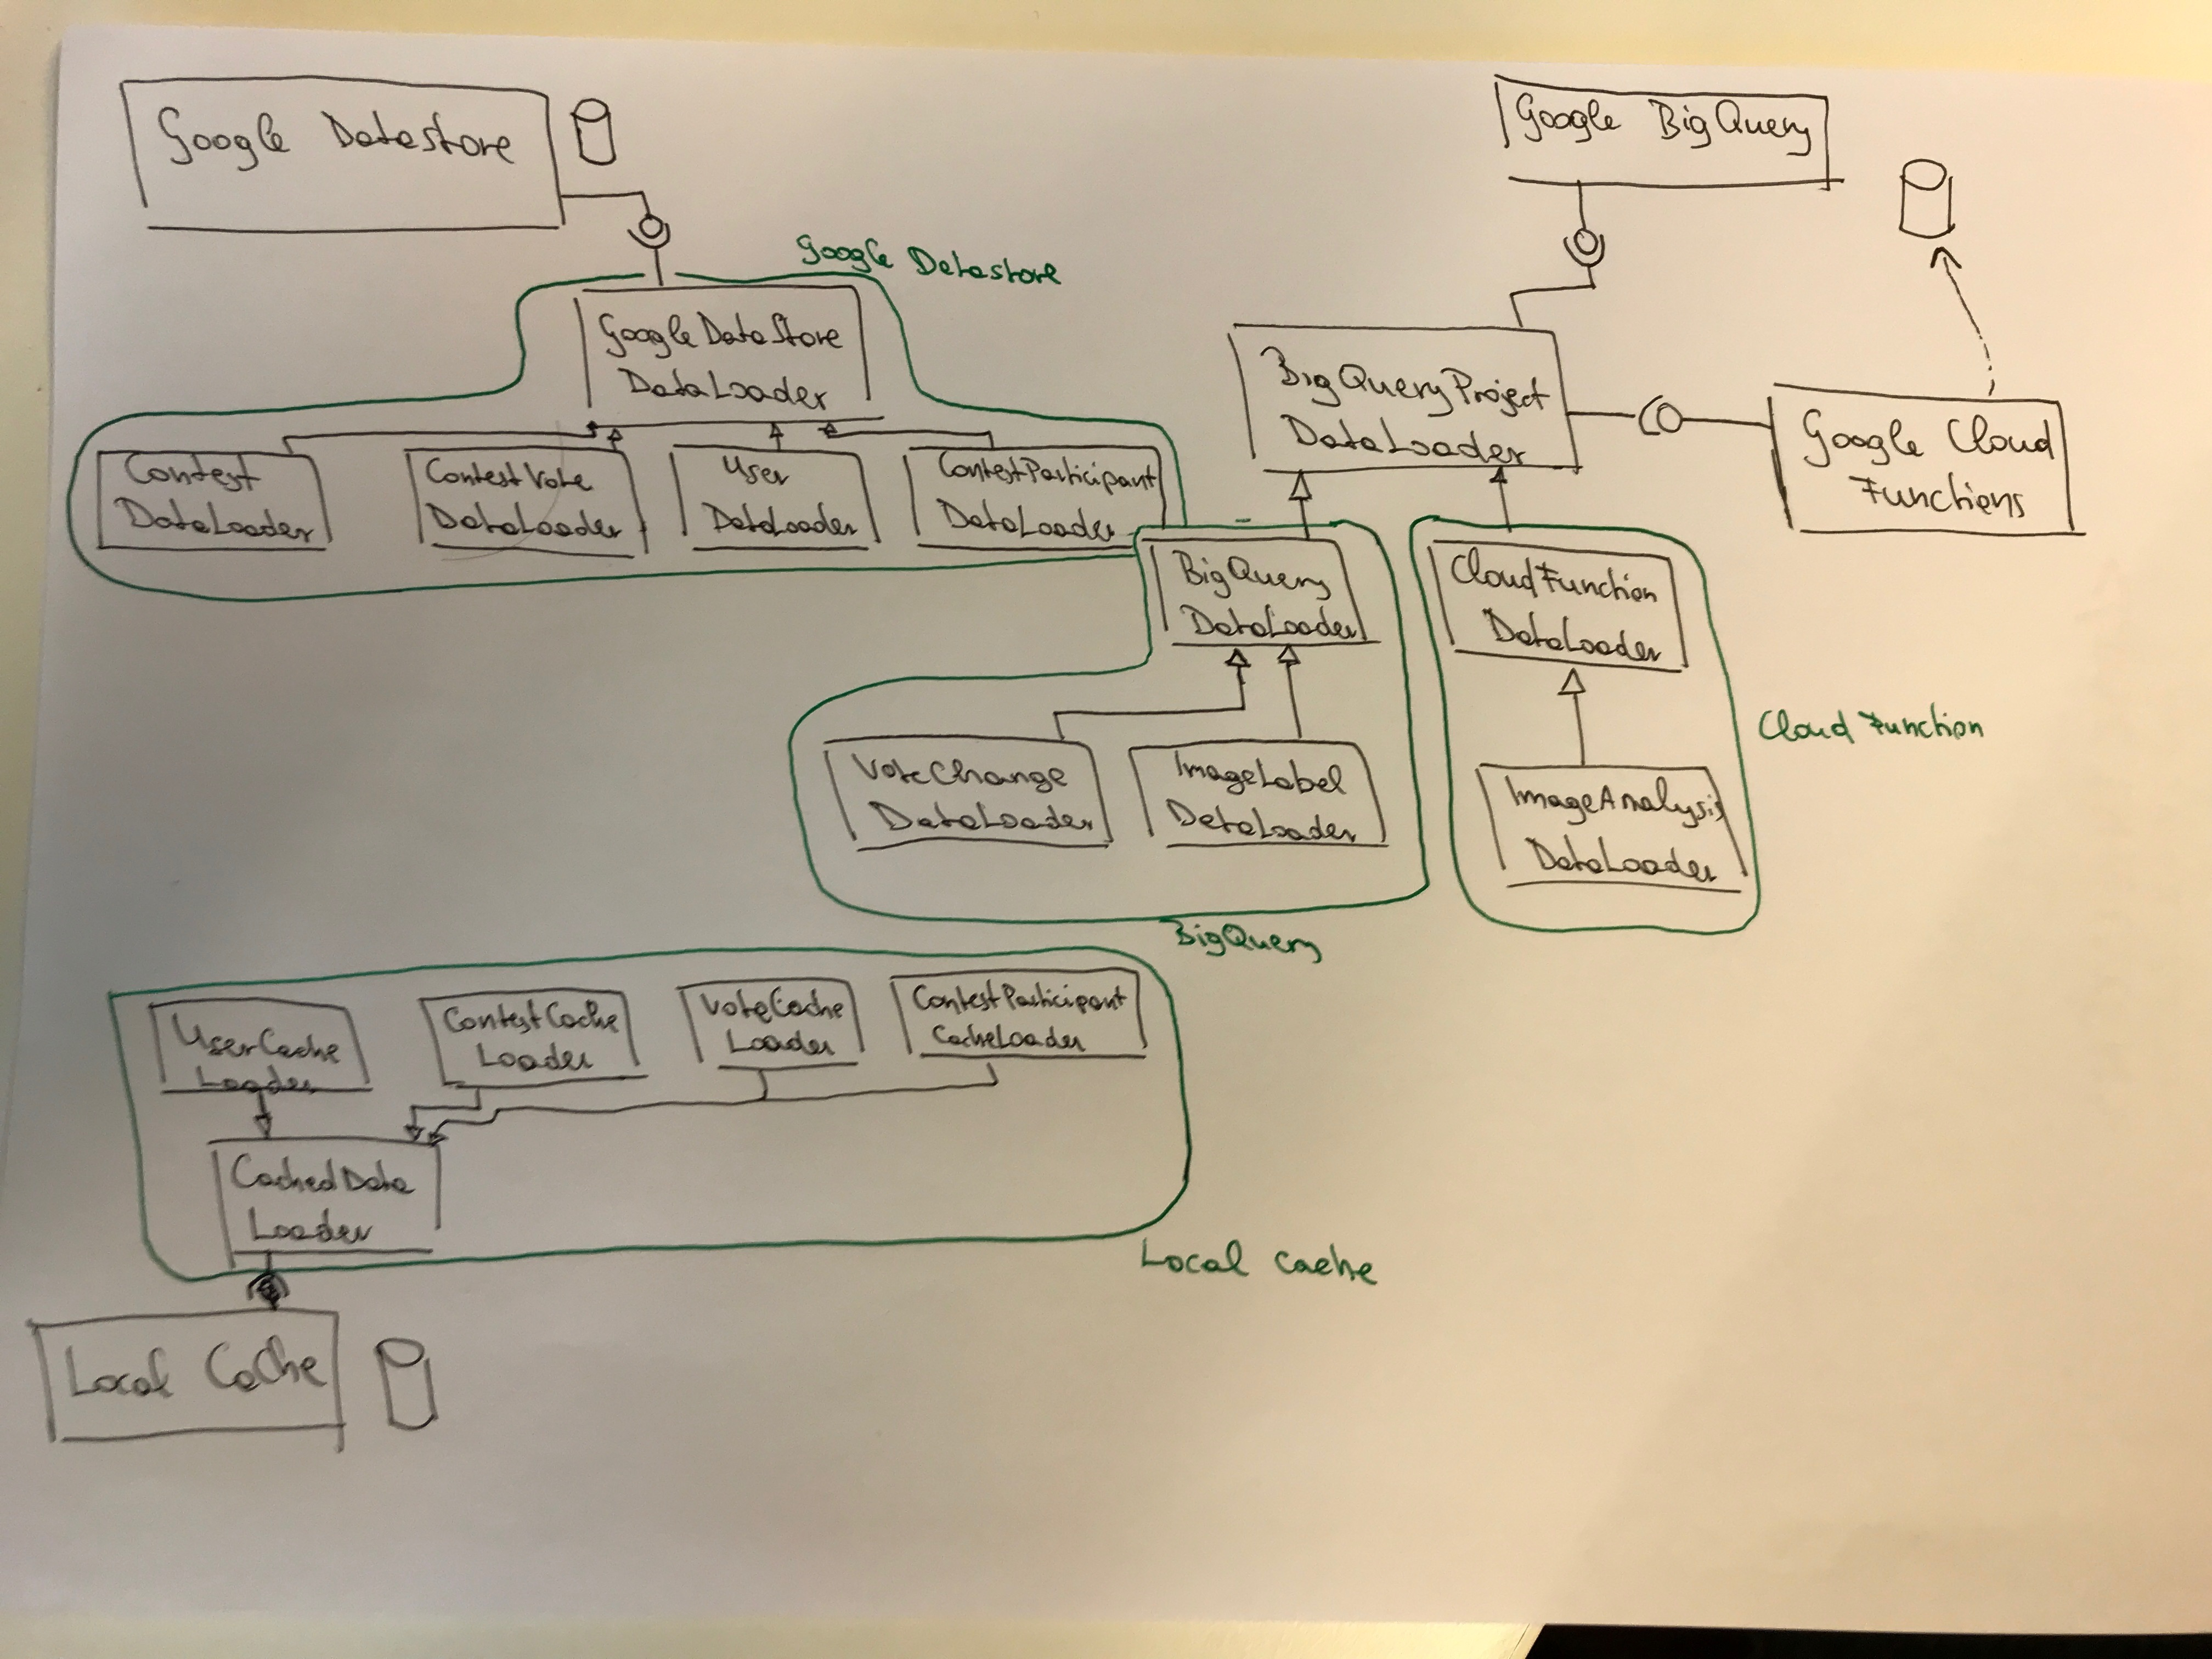
\includegraphics[width=0.8\textwidth]{Images/IMG_1317.jpg}
	% 		\caption{The data sources of the data analysis in the Choicely platform.}
	% 		\label{choicely_data_sources}
	% 	\end{center}
    % \end{figure}
    % \begin{figure}[h] 
	% 	\begin{center}
    %         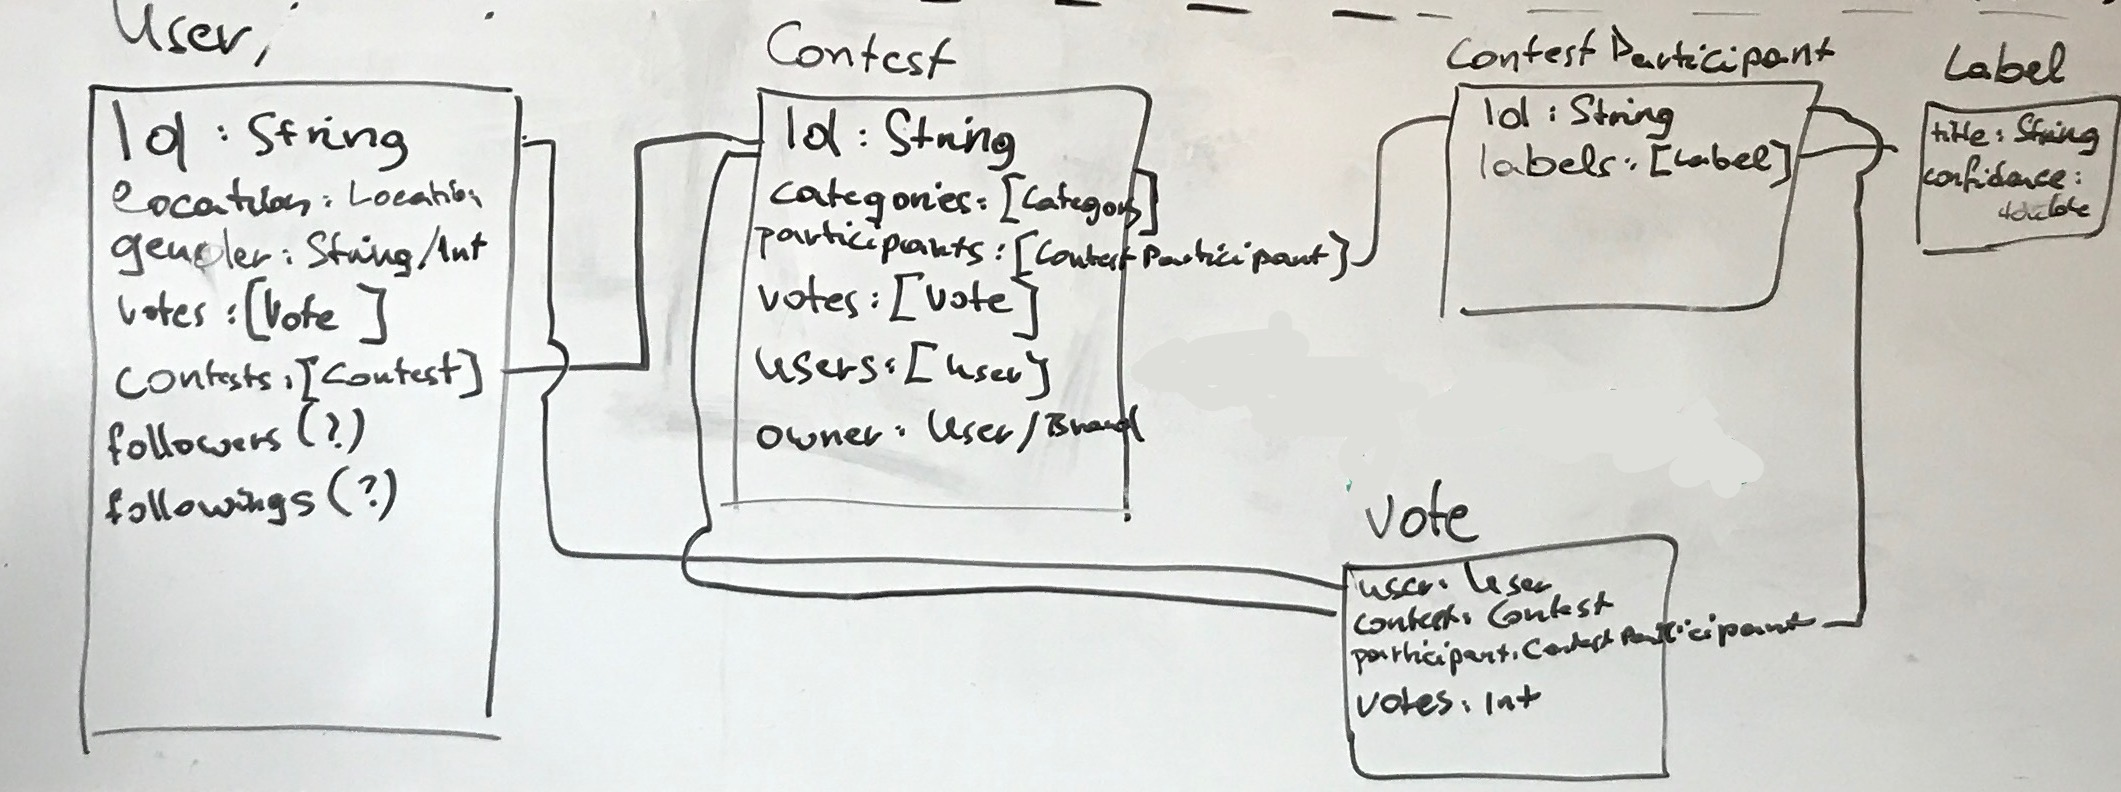
\includegraphics[width=0.8\textwidth]{Images/data_structure_whiteboard.jpg}
	% 		\caption{The structure of the data models of the Choicely platform.}
	% 		\label{choicely_data_models}
	% 	\end{center}
    % \end{figure}

    \subsection{Knowledge Discovery and Data Visualization}
    To answer RQ2 and RQ3 (presented in Chapter \ref{section::introduction}), the chosen methods presented in Chapter \ref{section::methodology} are applied in relation to Choicely's data. The paragraphs to follow elaborate a more in depth, what kind of data is used in case of the Choicely to answer the stated questions. On top of that it is explained, how the data was transformed in order to achieve the results. Data records collected before $1^{st}$ January, 2018 are used for the analyses. 

    % what is the goal of EDA? How is it used in this research? 
    The EDA fundamentally focused on two aspects of the data at hand: the user engagement in contests and the completeness of user profiles. In other words, the EDA is performed on the datasets extracted from the Contest, User and Vote entities in Choicely. 
    
    Contests have a few attributes which can help answering RQ2. To gain an understanding on how many users are typically engaged in contests, the number of unique voters is studied in comparison to the number of contests. The number of unique voters means the users, who have voted on at least one participant in a contest. This value can be retrieved for all contests in the platform. Contests can be filtered by their categories which is another approach towards finding answers to RQ2. Similarly to studying the number of unique voters over contests, the same metric is applied to all contest categories. By looking into how many users have voted in which kind of contests, one can get a grasp on the kind of contests that tend to attract more users.

    On top the number of unique voters, it can be studied what percentage of the users vote in more than one contest in a category. In other words, the return rate of users over categories can be studied to identify more engaging type of content. Accordingly, the Vote records are studied from the angle of voters and categories.

    To answer RQ3, Association Analysis using the Apriori algorithm is performed. In order to be able to execute the analysis, some preprocessing has to be done. The list of labels extracted from the participants in the contest are listed for each transaction alongside with the voters' demographic data. In other words, the data has to be transformed such that the input contains rows of the voters' demographic attributes and the computer-vision identified labels from the participants' images. In order to achieve this, the User, Contest, ImageLabel and Vote tables are joined together. The retrieved data is combined as shown in Table \ref{association_analyisis_data}. This data structure is adequate to perform the analysis on.
    
    \begin{table}[]
        \centering
        \begin{adjustbox}{width=1\textwidth}
            \begin{tabular}{l|l|l|l}
                gender & age group & country & labels \\
                \hline
                female & 25-34 & fin & ['fashion model', 'hair', 'model', 'beauty', '...] \\
                male & 18-24 & fin & ['dark hair', 'hair', 'model', 'smile', '...] \\
                male & 65+ & fin & ['fashion model', 'hair', 'shoulder', 'beauty', '...] \\
                female & 18-24 & swe & ['fashion model', 'hair', 'model', 'beauty', ...] \\
                male & 18-24 & hun & ['beauty', 'blond', 'human hair color', 'model', ...]
            \end{tabular}
        \end{adjustbox}
        \caption{The format of the data used for Association Analysis (the records dispalyed in the table are only examples).}
        \label{association_analyisis_data}
    \end{table}
    
    Using this approach, the support of the itemsets extracted from the labels can be calculated. The support in this case tells the percentage of votes, which were casted on a desired itemset. For instance, $S({"beauty", "blonde"}) = 0.6$ would mean that $60 \%$ of all votes were casted on participants whose images contained the ${"beauty", "blonde"}$ itemset. Likewise, if the list of vote transactions is filtered by one of the demographic attributes, the same can be said for the investigated group of users. 
    
    \begin{table}[]
        \centering
        \begin{adjustbox}{width=1\textwidth}
            \begin{tabular}{l|l|l}
                X & $S(X|gender=male)$ & $S(X|gender=female)$ \\
                \hline
                $\{"beauty", "blonde"\}$ & $0.3$ & $0.8$ \\
                $\{"bodybuilder", "muscle"\}$ & $0.6$ & $0.1$ \\
                $\{"sea", "photo shoot", "model"\}$ & $0.0$ & $1.0$
            \end{tabular}
        \end{adjustbox}
        \caption{The output format of the Association Analysis comparing genders, where X is the itemset and S is the support (the records dispalyed in the table are only examples).}
        \label{itemset_supports_format}
    \end{table}

    Figure \ref{association_analysis_flow} summarizes the flow of the Association Analysis. First, Computer Vision is applied on the participants images in order to automatically label the images with meta data. The demographic data from the users' profile, their vote transactions and the image labels are joined together to create the data structure presented in Table \ref{association_analyisis_data}. Next, the Apriori algorithm is applied to calculate the itemset supports (either on the full dataset or the transactions of a targeted group of users) as presented in Table \ref{itemset_supports_format}. 
    % Finally, Co-Clustering is utilized on the calculated supports 

    \begin{figure}[h] 
        \begin{center}
            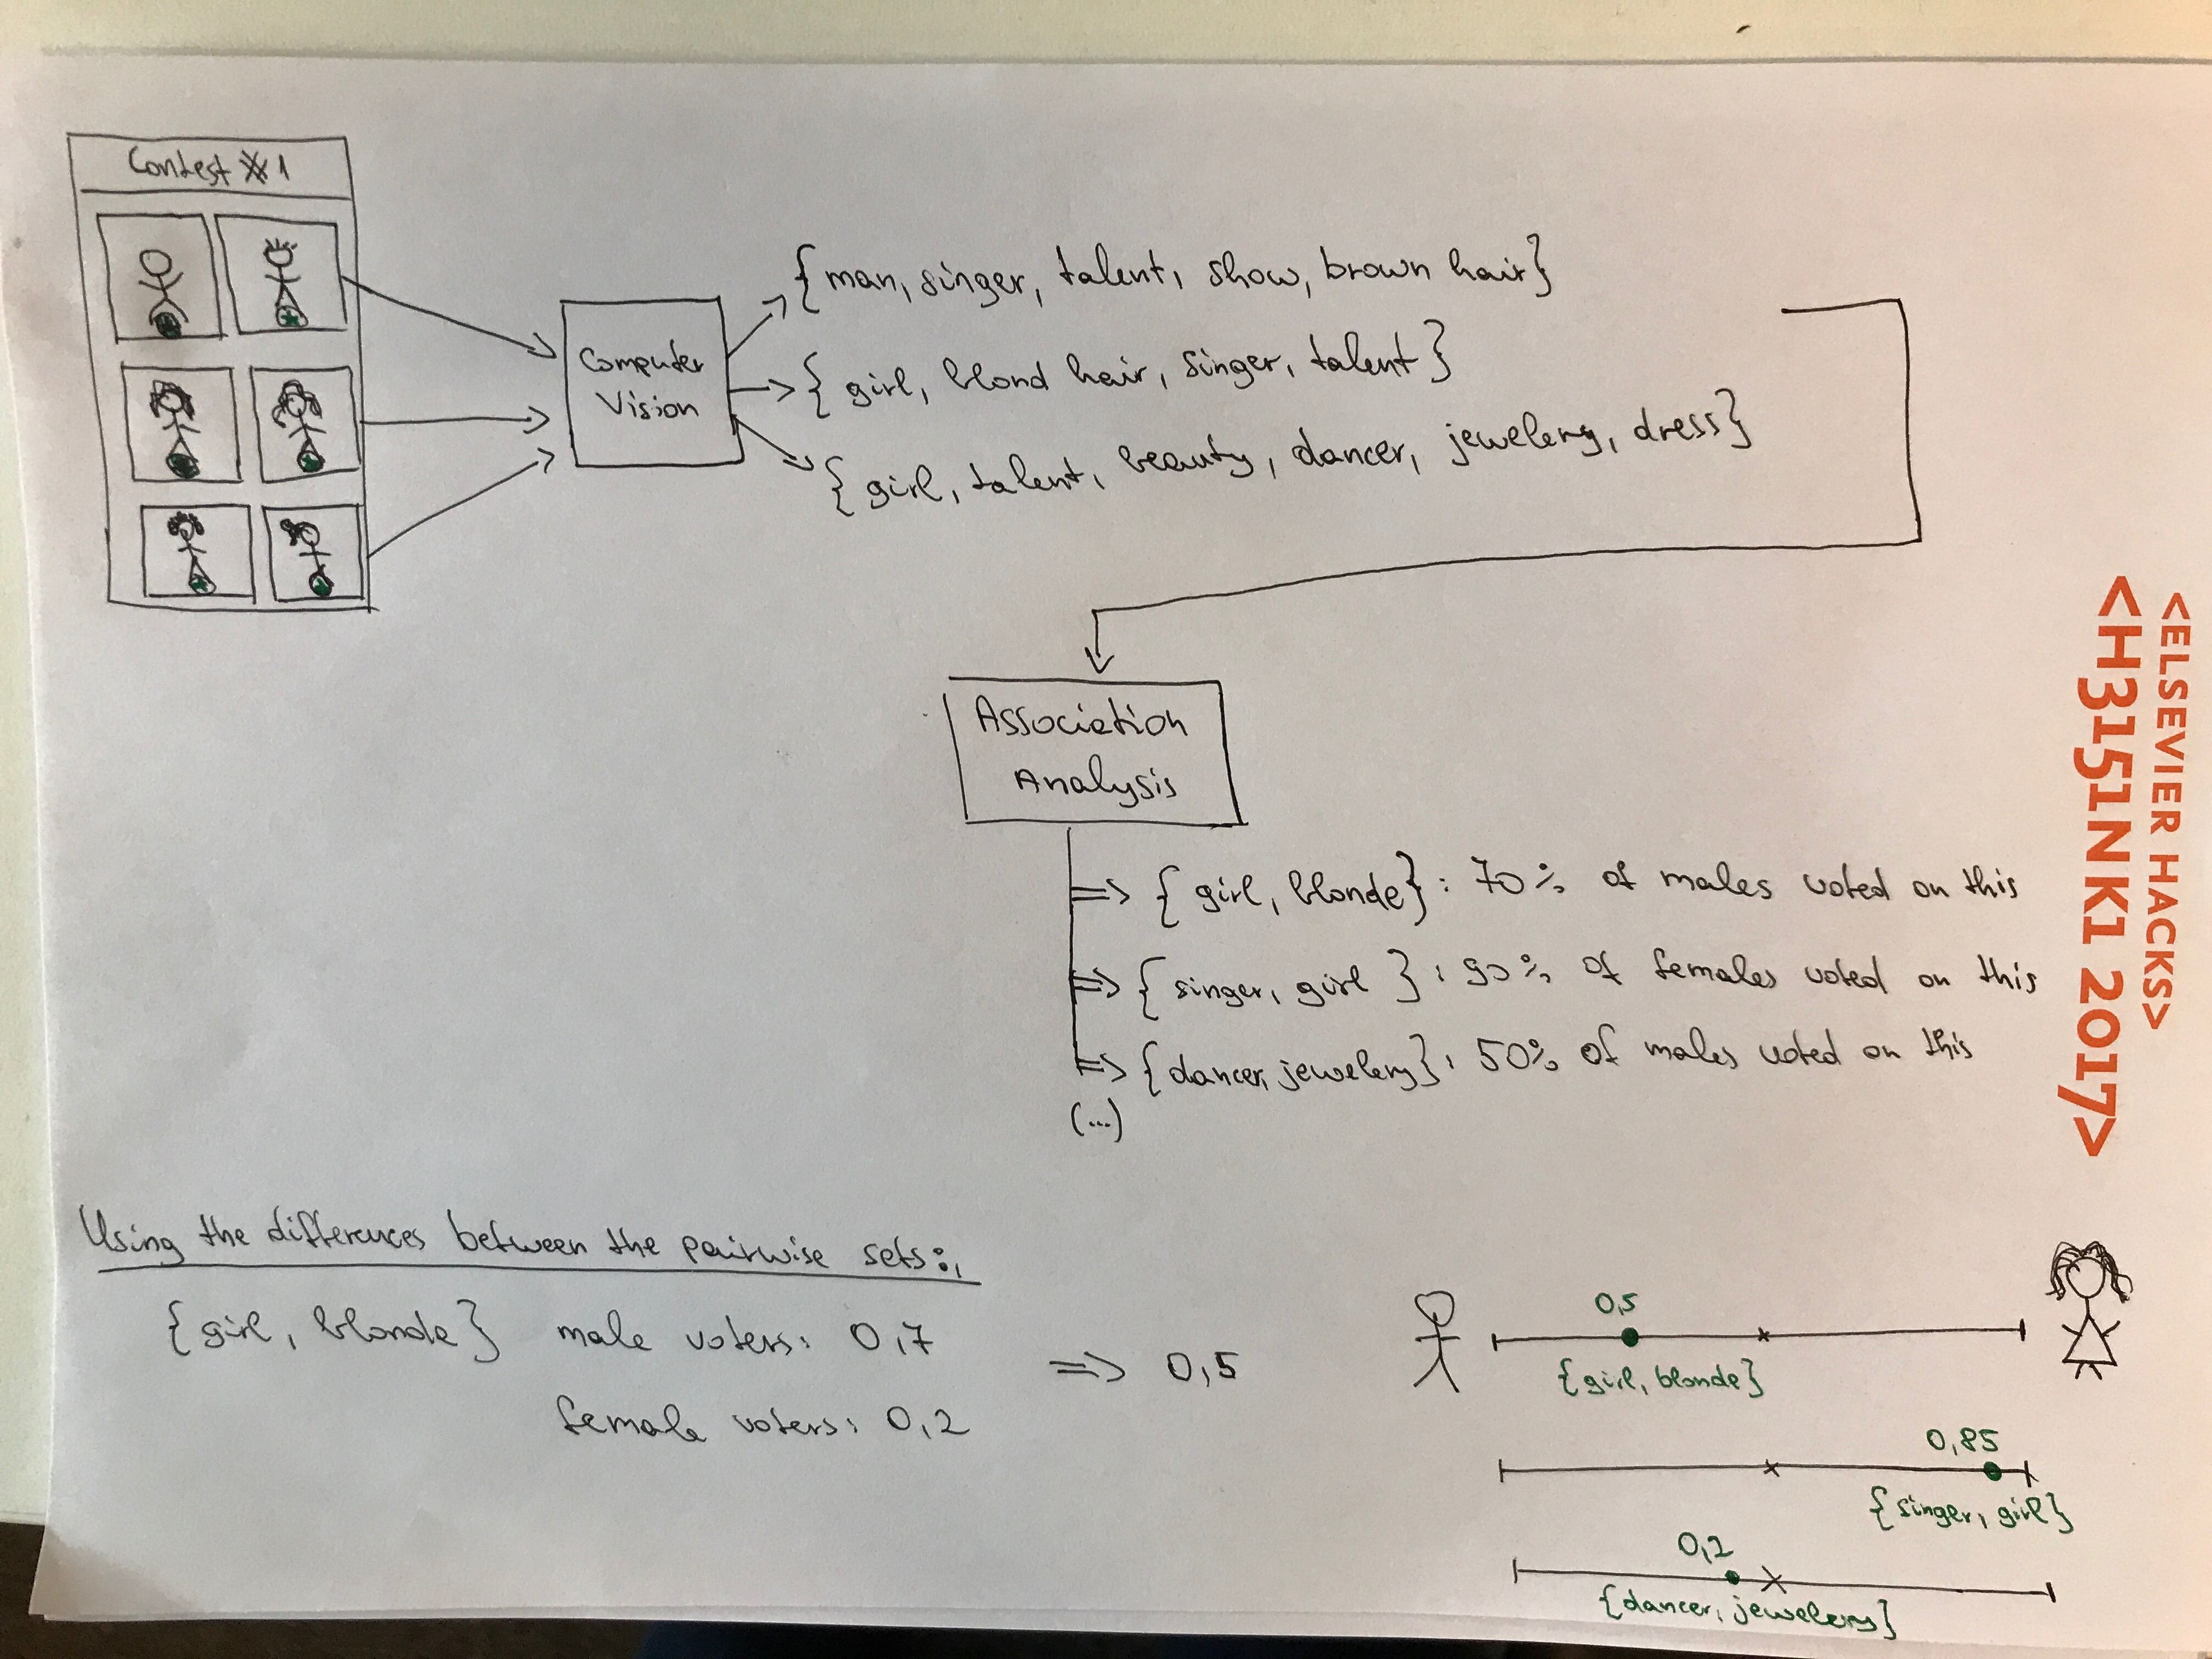
\includegraphics[width=0.8\textwidth]{Images/association_analysis_flow.jpg}
            \caption{The flow of the association analysis of the participants' images.}
            \label{association_analysis_flow}
        \end{center}
    \end{figure}